\documentclass{article}
\usepackage{graphicx}
\usepackage{wrapfig}
\usepackage{filecontents}
\usepackage{siunitx}
\usepackage[table]{xcolor}
\usepackage{float}
\usepackage{hyperref}

\usepackage{color} % balíček pro obarvování textů
\usepackage{xcolor}  % zapne možnost používání barev, mj. pro \definecolor
\usepackage{pgfplots} % http://www.chiark.greenend.org.uk/doc/texlive-doc/latex/pgfplots/pgfplots.pdf

\ifnum 0\ifxetex 1\fi\ifluatex 1\fi=0 % if pdftex
  \usepackage[T1]{fontenc}
  \usepackage[utf8]{inputenc}
\else % if luatex or xelatex
  \ifxetex
    \usepackage{mathspec}
  \else
    \usepackage{fontspec}
  \fi
  \defaultfontfeatures{Ligatures=TeX,Scale=MatchLowercase}
\fi
\usepackage[total={175mm,230mm}, top=23mm, left=20mm, includefoot]{geometry}
\hypersetup{
    colorlinks,
    linkcolor={blue!50!black},
    citecolor={green!50!black},
    urlcolor={blue!80!black}
}
% \definecolor{fialova}{RGB}{ 255, 000, 255}
\definecolor{color-si1}{RGB}{ 255, 000, 000}
\definecolor{color-si2}{RGB}{ 251, 130, 032}

\definecolor{color-ge1}{RGB}{ 000, 255, 000}
\definecolor{color-ge2}{RGB}{ 032, 251, 160}

\definecolor{color-inp1}{RGB}{ 000, 000, 255}
\definecolor{color-inp2}{RGB}{ 160, 032, 251}

\definecolor{color-geas1}{RGB}{ 225, 225, 000}
\definecolor{color-geas2}{RGB}{ 225, 225, 100}

\definecolor{sedak}{RGB}{ 100, 100, 100}


\newcommand \obr[1]
{ obr.~\ref{#1}}

\newcommand \tab[1]
{ tab.~ß\ref{#1}}


\begin{document}

\pagestyle{empty}

\definecolor{color_29791}{rgb}{0,0,0}
\begin{figure}[H]
    \hspace{-13mm}
    \begin{minipage}[t]{\textwidth}
        \vspace{-20mm}
        \begin{tikzpicture}[overlay]
            \path(0pt,0pt);
        \end{tikzpicture}
        \begin{picture}(-5,0)(2.5,0)
            \put(123.656,-82.75397){\fontsize{18}{1}\usefont{T1}{ptm}{m}{n}\selectfont\color{color_29791}VYSOKÉ UČENÍ TECHNICKÉ V BRNĚ}
            \put(76.296,-104.785){\fontsize{13}{1}\usefont{T1}{ptm}{m}{n}\selectfont\color{color_29791}FAKULTA  ELEKTROTECHNIKY A KOMUNIKAČNÍCH TECHNOLOGIÍ}
            \put(198.447,-128.5339){\fontsize{16}{1}\usefont{T1}{cmr}{b}{n}\selectfont\color{color_29791}Ústav elektrotechnologie}
            \put(156.848,-278.1589){\fontsize{14}{1}\usefont{T1}{ptm}{m}{n}\selectfont\color{color_29791}LABORATORNÍ CVIČENÍ Z PŘEDMĚTU}
            \put(108.123,-300.2579){\fontsize{14}{1}\usefont{T1}{cmr}{b}{n}\selectfont\color{color_29791}VYBRANÉ PARTIE Z OBNOVITELNÝCH ZDROJŮ A}
            \put(173.123,-320.2579){\fontsize{14}{1}\usefont{T1}{cmr}{b}{n}\selectfont\color{color_29791}UKLÁDÁNÍ ENERGIE (BPC-OZU)}
            \put(55.85,-421.25){\fontsize{14}{1}\usefont{T1}{cmr}{b}{n}\selectfont\color{color_29791}Číslo úlohy: 7}
            \put(55.85,-469.547){\fontsize{14}{1}\usefont{T1}{cmr}{b}{n}\selectfont\color{color_29791}Název úlohy: Využití termoelektrického jevu pro získávání energie}
            \put(23.9,-620.32){\fontsize{12}{1}\usefont{T1}{cmr}{b}{n}\selectfont\color{color_29791}Jméno a příjmení, ID:}
            \put(23.9,-637.119){\fontsize{12}{1}\usefont{T1}{cmr}{b}{n}\selectfont\color{color_29791}Tomáš Vavrinec, 240893}
            \put(186.95,-620.32){\fontsize{12}{1}\usefont{T1}{cmr}{b}{n}\selectfont\color{color_29791}Atmosférický tlak:}
            \put(186.95,-637.119){\fontsize{12}{1}\usefont{T1}{cmr}{b}{n}\selectfont\color{color_29791}1018 hPa}
            \put(293.25,-620.32){\fontsize{12}{1}\usefont{T1}{cmr}{b}{n}\selectfont\color{color_29791}Teplota okolí: }
            \put(293.25,-637.119){\fontsize{12}{1}\usefont{T1}{cmr}{b}{n}\selectfont\color{color_29791}21.7°C}
            \put(417.25,-620.32){\fontsize{12}{1}\usefont{T1}{cmr}{b}{n}\selectfont\color{color_29791}Relativní vlhkost:}
            \put(417.25,-637.119){\fontsize{12}{1}\usefont{T1}{cmr}{b}{n}\selectfont\color{color_29791}24.6\%}
            \put(23.9,-665.77){\fontsize{12}{1}\usefont{T1}{cmr}{b}{n}\selectfont\color{color_29791}Měřeno dne:}
            \put(23.9,-682.569){\fontsize{12}{1}\usefont{T1}{cmr}{b}{n}\selectfont\color{color_29791}25.2.2023}
            \put(186.95,-665.77){\fontsize{12}{1}\usefont{T1}{cmr}{b}{n}\selectfont\color{color_29791}Odevzdáno dne:}
            \put(293.25,-665.77){\fontsize{12}{1}\usefont{T1}{cmr}{b}{n}\selectfont\color{color_29791}Ročník, stud. skupina:}
            \put(293.25,-682.569){\fontsize{12}{1}\usefont{T1}{cmr}{b}{n}\selectfont\color{color_29791}2}
            \put(417.25,-665.77){\fontsize{12}{1}\usefont{T1}{cmr}{b}{n}\selectfont\color{color_29791}Kontrola:}
            \put(23.9,-703.42){\fontsize{12}{1}\usefont{T1}{cmr}{b}{n}\selectfont\color{color_29791}Spolupracovali:}
            \put(23.9,-720.219){\fontsize{12}{1}\usefont{T1}{cmr}{b}{n}\selectfont\color{color_29791}Kateřina Koudelková}
        \end{picture}
        \begin{tikzpicture}[overlay]
            \path(0pt,0pt);
            \draw[color_29791,line width=0.5pt]
            (20.4pt, -606.117pt) -- (20.4pt, -722.815pt)
            ;
            \draw[color_29791,line width=0.5pt]
            (183.45pt, -606.117pt) -- (183.45pt, -651.067pt)
            ;
            \draw[color_29791,line width=0.5pt]
            (183.45pt, -651.567pt) -- (183.45pt, -688.717pt)
            ;
            \draw[color_29791,line width=0.5pt]
            (289.75pt, -606.117pt) -- (289.75pt, -651.067pt)
            ;
            \draw[color_29791,line width=0.5pt]
            (289.75pt, -651.567pt) -- (289.75pt, -688.717pt)
            ;
            \draw[color_29791,line width=0.5pt]
            (413.75pt, -606.117pt) -- (413.75pt, -651.067pt)
            ;
            \draw[color_29791,line width=0.5pt]
            (413.75pt, -651.567pt) -- (413.75pt, -688.717pt)
            ;
            \draw[color_29791,line width=0.5pt]
            (544.9pt, -606.117pt) -- (544.9pt, -722.815pt)
            ;
            \draw[color_29791,line width=0.5pt]
            (20.15pt, -605.867pt) -- (545.15pt, -605.867pt)
            ;
            \draw[color_29791,line width=0.5pt]
            (20.65pt, -651.317pt) -- (544.65pt, -651.317pt)
            ;
            \draw[color_29791,line width=0.5pt]
            (20.65pt, -688.967pt) -- (544.65pt, -688.967pt)
            ;
            \draw[color_29791,line width=0.5pt]
            (20.15pt, -723.065pt) -- (545.15pt, -723.065pt)
            ;
            \draw[color_29791,line width=1.5pt]
            (15.75pt, -15.59998pt) -- (15.75pt, -729pt)
            ;
            \draw[color_29791,line width=1.5pt]
            (549.55pt, -15.59998pt) -- (549.55pt, -729pt)
            ;
            \draw[color_29791,line width=1.5pt]
            (15.75pt, -729pt) -- (549.55pt, -729pt)
            ;
            \draw[color_29791,line width=1.5pt]
            (15pt, -14.84998pt) -- (550.3pt, -14.84998pt)
            ;
        \end{tikzpicture}
    \end{minipage}
\end{figure}

\newpage
\pagestyle{plain}




\begin{figure}
  \begin{minipage}[t]{\textwidth}
    \section*{Zadání}
    \begin{enumerate}
    \item V úloze jsou použity superkondenzátory od tří různých výrobců (Eaton, Maxwell, Nichicon) se stejnou hodnotou nominální kapacity a napětí. Jejich technické listy naleznete v příloze. Vypište z technických listů a porovnejte následující parametry udávané jednotlivým výrobci:
    \begin{itemize}
      \item Vnitřní sériový odpor RESR
      \item Maximální proud IMAX
      \item Unikající proud (tzv. Leakage Current) IL
    \end{itemize}
    \item U vybraných superkondezátorů změřte jejich kapacitu C pomocí vybíjecí metody a porovnejte s nominální kapacitou udávanou výrobcem.
    \item U vybraných superkondezátorů změřte hodnotu vnitřního sériového odporu RESR a porovnejte s hodnotami běžných kondenzátorů. A porovnejte s hodnotami udávanými výrobcem.
    \item Změřte u vybraných superkondenzátorů velikost svodového proudu IL. Vypočtěte a do protokolu uveďte hodnotu energie uložené v superkondenzátoru pro hodnoty napětí 2.5 V, 2 V, 1 V a 0.5 V.
    \end{enumerate}
  \end{minipage}
    
  \section*{Teoretický úvod a jednotlivá měření}
  \begin{minipage}[t]{0.49\textwidth}
    \vspace{-35mm}
    Pro naše měření budeme předpokládat model Kondenzátoru se dvěma odpory.
    V ideálním případě tedy \(R_P = \infty \) a \(R_{ESR} = 0\)
  \end{minipage}
  \begin{minipage}[t]{0.49\textwidth}
    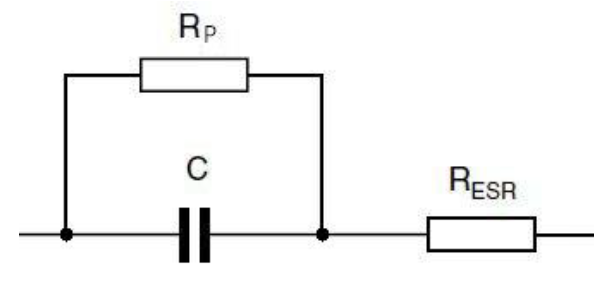
\includegraphics[width=\textwidth]{model.png}
  \end{minipage}
\end{figure}

\subsection*{Měření \(R_{ESR}\)}
Měření sériového odporu je možné pomocí tzv. vybíjecí metody, u které k nabitému kondenzátoru připojíme zatěžovací rezistor o známém odporu \(R_{SENS}\), který nám společně s virtuálním odporem \(R_{ESR}\) vytvoří napěťový dělič.
Pokud, pak budeme tento rezistor střídavě připojovat a odpojovat, na výstupu se nám ukáže obdélníkový signál, z jehož amplitudy \(U_{AMP}\) a minimálního napětí \(U_{MIN}\) lze určit hodnotu \(R_{ESR}\). 
\\ \\
\Large
\(
  R_{ESR} = \frac{U_{AMP}\cdot R_{SENS}}{U_{MIN}}
\)
\normalsize
\\ \\
\begin{figure}[H]
  \begin{minipage}[t]{\textwidth}
    \subsubsection*{Naše měření}
    Každý z kondenzátoru byl nabit na \(U_{AMP} = 2.2\-[V]\) a zatěžovací rezistor \(R = 2\-[\Omega]\)
    \begin{table}[H]
      \centering
      % \vspace{-75mm}
      \begin{tabular}{|c|c|c|c||c|}
      \hline
                  &	\(U_{MIN}\-[V]\)  & \(U_{AMP}\-[mV]\)  & \(R_{ESR}\-[m\Omega]\) & katalogová hodnota \(R_{ESR}\-[m\Omega]\)  \\ \hline
        Maxwell   & 2.038             & 162.5              & 159.5                  & \(R_{ESR} <  75\)                          \\ \hline
        Eaton     & 2.040             & 160.0              & 156.9                  & \(R_{ESR} <  34\)                          \\ \hline
        Nichicon  & 2.035             & 165.0              & 162.2                  & \(R_{ESR} < 250\)                          \\ \hline
      \end{tabular}
      \caption{\label{ESR} Změřené, vypočtené a výrobcem určené hodnoty k úkolu 1}
    \end{table}
    \vspace{-5mm}
    Příklad výpočtu:
    \\ \\
    \Large
    \(
      R_{ESR} = \frac{U_{AMP}\cdot R_{SENS}}{U_{MIN}} = \frac{162.5\cdot10^{3}\cdot 2}{2.038}\-[\Omega] = 0.1595\-[\Omega] = 159.5\-[m\Omega]
    \)
    \normalsize
    \\ \\
    Naše měření bylo buď zatíženo podstatnou chybou metody nebo je skutečný odpor kondenzátorů \(R_{ESR}\) velmi výrazně nad limity stanovenými výrobcem. 
  \end{minipage}
\end{figure}

\subsection*{Měření kapacity \(C\)}
Kapacitu kondenzátoru lze změřit pomocí měření průběhu jeho napětí při jeho vybíjení známým proudem.
Pro jednoduchost tedy použijeme zdroj konstantního proudu o hodnotě \(I = 1\-[A]\) a následně na změřeném průběhu vybereme lineární část vybíjení (tedy tu kde se kondenzátor skutečně vybíjel požadovaným proudem).
Kapacitu kondenzátoru můžeme následně určit jako:
\\ \\
\Large
\(
  C = \frac{t\cdot \Delta U}{I}
\)
\normalsize
\\ \\

\begin{figure}[H]
  \begin{minipage}[t]{\textwidth}
    \subsubsection*{Naše měření}
    Pro všechny kondenzátory byl vybíjecí proud \(I = 1\-[A]\)
    \begin{table}[H]
      % \vspace{-75mm}
      \centering
      \begin{tabular}{|c|c|c||c|c|}
        \hline
                    &	\(\Delta U\-[V]\)  & \(t\-[s]\)   & \(C\-[F]\)  & katalogová hodnota \(C\)  \\ \hline
          Maxwell   & 1.00               & 9.48         & 9.48        & \(8 \leq C \leq 10\)      \\ \hline
          Eaton     & 1.00               & 8.36         & 8.36        & \(9 \leq C \leq 13\)      \\ \hline
          Nichicon  & 1.00               & 8.4          & 8.4         & \(8 \leq C \leq 12\)      \\ \hline
      \end{tabular}
      \caption{\label{C} Změřené, vypočtené a výrobcem určené hodnoty k úkolu 2}
    \end{table}
    Příklad výpočtu:
    \\ \\
    \Large
    \(
      C = \frac{t\cdot \Delta U}{I} = \frac{9.48 \cdot 1}{1}\-[F]=9.48\-[\Omega]
    \)
    \normalsize
    \\ \\
    Z našeho měření kapacity plyne, že kapacita kondenzátorů je v toleranci určené výrobcem u kondenzátorů Maxwell a Nichicon, zatím co kondenzátor Eaton pravděpodobně vlivem stáří svojí kapacitu snížil pod úroveň výrobcem určeného intervalu.  
  \end{minipage}
\end{figure}

\subsection*{Měření paralelního odporu \(R_P\)}
Paralelní odpor způsobuje vybíjení kondenzátoru proudem \(I_L\).
Hodnotu \(I_L\) můžeme určit z poklesu napětí na odporu, ze kterého není odebírán žádný proud za čas \(t\).
\(I_L\) tak můžeme určit jako:
\\ \\
\Large
\(
  I_L = \frac{C\cdot \Delta U}{t}
\)
\normalsize
\\ \\

\begin{figure}[H]
  \begin{minipage}[t]{\textwidth}
    \subsubsection*{Naše měření}
    Každý z kondenzátorů byl nabit na \(U_{AMP} = 2.2\-[V]\) a ponechán v nepřipojeném stavu po dobu 15 minut
    \begin{table}[H]
      % \vspace{-75mm}
      \centering
      \begin{tabular}{|c|c|c||c|c|}
      \hline
                  &	\(U\-[V]\) & \(I_L \-[mA]\) & katalogová hodnota \(I_L\-[mA]\)  \\ \hline
        Maxwell   & 2.144      & 0.590          & 0.030                             \\ \hline
        Eaton     & 2.067      & 1.235          & 0.023                             \\ \hline
        Nichicon  & 2.072      & 1.195          & 5                                 \\ \hline
      \end{tabular}
      \caption{\label{U_AMP} Změřené, vypočtené a výrobcem určené hodnoty k úkolu 3}
    \end{table}
    Příklad výpočtu:
    \\ \\
    \Large
    \(
      I_L = \frac{C\cdot \Delta U}{t} = \frac{9.48\cdot 0.56}{15\cdot 60}\-[A]=0.0005899\-[A] = 0.5899\-[mA]
    \)
    \normalsize
    \\ \\
    Z našeho měření plyne, že jen kondenzátor Nichicon má hodnotu \(I_L\) v toleranci určené výrobcem zatím co u kondenzátorů Maxwell a Eaton jsme naměřili svodový proud řádově vyšší.
    Vzhledem k velké odchylce od katalogové hodnoty je pravděpodobné, že došlo k chybě měření.  
  \end{minipage}
\end{figure}

\subsection*{Závěr}

\begin{figure}[H]
  \begin{minipage}[t]{\textwidth}
    \begin{table}[H]
      \vspace{-10mm}
      \centering
      \begin{tabular}{|c|c|c|c|}
        \hline
                    & \(R_{ESR}\-[m\Omega]\) & \(C\-[F]\) & \(I_L \-[mA]\) \\ \hline
          Maxwell   & 159.5                  & 9.48       & 0.590          \\ \hline
          Eaton     & 156.9                  & 8.36       & 1.235          \\ \hline
          Nichicon  & 162.2                  & 8.4        & 1.195          \\ \hline
      \end{tabular}
      \caption{\label{Vysledky} Výsledky měření}
    \end{table}
    \vspace{-10mm}
  \end{minipage}
\end{figure}

\subsection*{Měření \(R_{ESR}\)}
Naše měření bylo buď zatíženo podstatnou chybou metody nebo je skutečný odpor kondenzátorů \(R_{ESR}\) velmi výrazně nad limity stanovenými výrobcem. 
\subsection*{Měření kapacity \(C\)}
Z našeho měření kapacity plyne, že kapacita kondenzátorů je v toleranci určené výrobcem u kondenzátorů Maxwell a Nichicon, zatím co kondenzátor Eaton pravděpodobně vlivem stáří svojí kapacitu snížil pod úroveň výrobcem určeného intervalu.
\subsection*{Měření paralelního odporu \(R_P\)}
Z našeho měření plyne že jen kondenzátor Nichicon má hodnotu \(I_L\) v toleranci určené výrobcem zatím co u kondenzátorů Maxwell a Eaton jsme naměřili svodový proud řádově vyšší.
Vzhledem k velké odchylce od katalogové hodnoty je pravděpodobné, že došlo k chybě měření.

\end{document}